\begin{figure}[H]
    \centering
    
\includegraphics[angle=90, height=610pt, 
    width=\textwidth]{hpSaetze1.PNG}
    \caption*{Auflistung der H- und P- Sätze Teil 1 \cite{baua}}
    \label{fig:hpsaetze1}
\end{figure}

\begin{figure}[H]
    \centering
    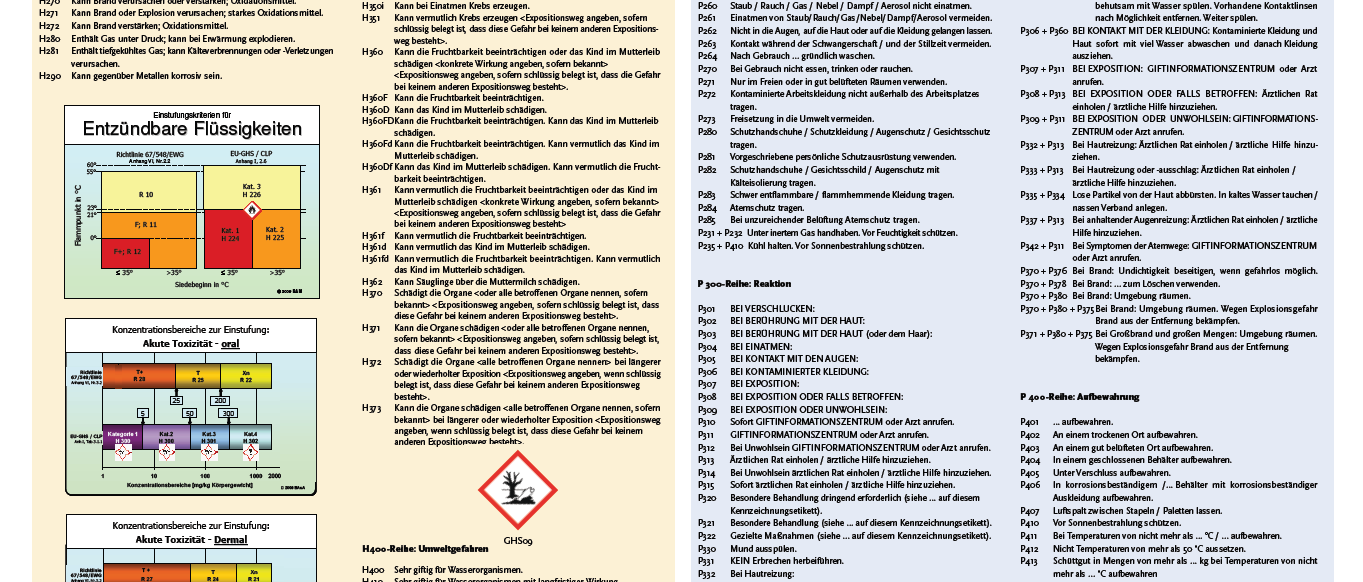
\includegraphics[angle=90, height=640pt, 
    width=\textwidth]{hpSaetze22.PNG}
    \caption*{Auflistung der H- und P- Sätze Teil 2 \cite{baua}}
    \label{fig:hpsaetze2}
\end{figure}

\begin{figure}[H]
    \centering
    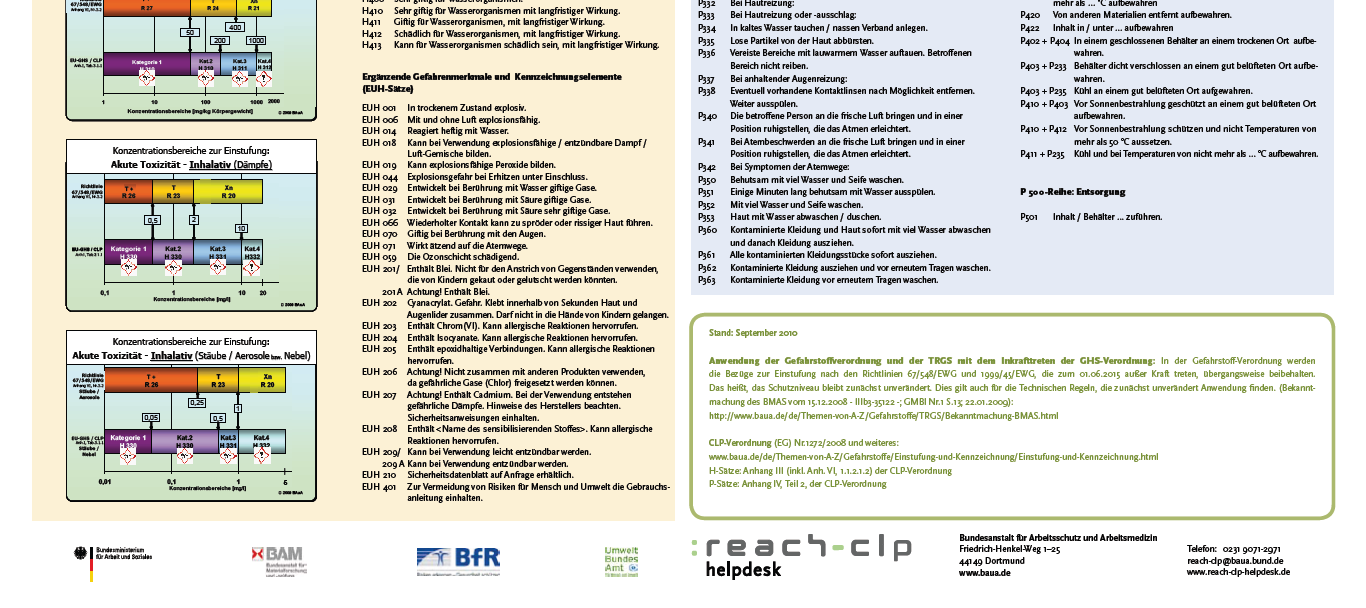
\includegraphics[angle=90, height=640pt, 
    width=\textwidth]{hpSaetze32.PNG}
    \caption*{Auflistung der H- und P- Sätze Teil 3 \cite{baua}}
    \label{fig:hpsaetze3}
\end{figure}
